% simple.tex - A simple article to illustrate my intermediary report.

%preamble

\documentclass[12pt]{article}
\usepackage[english]{babel}
\usepackage{amsmath,amsthm}
\usepackage{amsfonts}
\usepackage{url}
\usepackage{hyperref}
\hypersetup{colorlinks=true}
\usepackage{times}
\usepackage{latexsym}
\usepackage{graphicx}
\usepackage{listings}

\begin{document}

%top matter

\title{Num\u{a}rul Cromatic \\}
\author{Cristina Bivolan}
\date{\today}
\maketitle

\begin{tabbing}
\indent{Profesor:}  \=\href{http://software.ucv.ro/~cbadica}{Costin B\u{a}dic\u{a}} \\
\indent{Profesor laborator:}  \=\href{http://www.becheru.net/}{Alex Becheru} \\
\end{tabbing}

% abstract

\begin{abstract}
 Acest document introduce metodologia de dezvoltare a unei librarii pentru colorarea unui graf neorientat si determinarea numarului cromatic (\href{https://en.wikipedia.org/wiki/Graph_coloring}{Graph coloring}). Documentul contine,de asemenea,si descrierea tuturor variabilelor si functiilor folosite pentru a duce la bun sfarsit cerinta problemei. Tinta acestui proiect: studentii din anul $I$,specializarea Calculatoare.
\end{abstract}

\begin{quote}
\indent{Precizari:}
\end{quote}

\begin{itemize}
  \item Specializarea : Calculatoare cu predare in limba Romana
  \item Anul : $I$
  \item Grupa : 1.1 A
\end{itemize}

\vfill

\thanks{Universitatea din Craiova,Facultatea de Automatica,Calculatoare si Electronica.}

\pagebreak

%sections

\section{Cerinta problemei}
Scopul acestui proiect este de a implementa doi algoritmi diferiti pentru aflarea numarului cromatic al unui graf neorientat.Marimea grafului cat si a matricei de adiacenta va fi alocata dinamic pentru a folosi economic memoria.De asemenea,vor fi create functii pentru rezolvarea problemei folosing algoritmul Greedy, si pentru algoritmul Backtracking.


\section{Pseudocodul}
\begin{center}
\begin{tabbing}

FUNCTIA-Greedy($graf$) \\
1.\indent \ \ \ \ \ \ \ \ \  $i,j$\\
2.\indent \ \ \ \ \ \ \ \ \  $VectorCulori - colors$\\
3.\indent \ \ \ \ \ \ \ \ \  $NrMinCulori -  minColors$\\
4.\indent \ \ \ \ \ \ \ \ \ {\bf pentru}  i \leftarrow 1,nrNoduri,i \leftarrow  i \rightarrow next \\
4.1.\indent \ \ \ \ \ \ \ \ \ \ \ $colors[i]$ \leftarrow $1$\\
4.2.\indent \ \ \ \ \ \ \ \ \ \ \ \ \  {\bf pentru} $i$ \leftarrow $1,nrNoduri,i$ \leftarrow i\rightarrow $next$ \\
4.2.1.\indent \ \ \ \ \ \ \ \ \ \ \ \ \ \ \ \  {\bf daca} $grafAdjMatr[i][j]=1$ {\bf si} $colors[i]=colors[j]$  {\bf atunci} \\
4.2.1.1\indent \ \ \ \ \ \ \ \ \ \ \ \ \ \ \ \ \ \ $colors[i] \leftarrow colors[j]+1$ \\
4.2.1.2\indent \ \ \ \ \ \ \ \ \ \ \ \ \ \ \ \ \ \ $minColors \leftarrow colors[j]+1$ \\
\end{tabbing}
\end{center}

\begin{center}
\begin{tabbing}
FUNCTIA-Printeaza($colors,graf$) \\
1.\indent \ \ \ \ \ \ \ \ \  $i$\\
2.\indent \ \ \ \ \ \ \ \ \  $NrMinCulori -  minColors$\\
3.\indent \ \ \ \ \ \ \ \ \ {\bf pentru} $i$ \leftarrow $1$,$nrNoduri$,$i$ \leftarrow i \rightarrow $next$ \\
3.1.\indent \ \ \ \ \ \ \ \ \ \ \ \textbf{scrie} $nodul\ i \ are \ culoarea \ colors[i]$\\
3.2.\indent \ \ \ \ \ \ \ \ \ \ \ \ \ \ \ \  {\bf daca} $colors[i]>minColors$  {\bf atunci} \\
3.2.1.\indent \ \ \ \ \ \ \ \ \ \ \ \ \ \ \ \ \ \ $minColors \leftarrow colors[i]$ \\

\end{tabbing}
\end{center}


\begin{center}
\begin{tabbing}
FUNCTIA-Verificare($nod,graf,colors,culoare$) \\
1.\indent \ \ \ \ \ \ \ \ \  $i,j$\\
2.\indent \ \ \ \ \ \ \ \ \ {\bf pentru} $i$ \leftarrow $1$,$nrNoduri$,$i$ \leftarrow i \rightarrow $next$ \\
2.1.\indent \ \ \ \ \ \ \ \ \ \ \ \ \ \  {\bf daca} $grafAdjMatr[nod][i]=1$ {\bf si} $culoare=colors[i]$   {\bf atunci} \\
2.1.1.\indent \ \ \ \ \ \ \ \ \ \ \ \ \ \ \ \ \textbf{returneaza} $0$\\
3.\indent \ \ \ \ \ \ \ \ \ \textbf{returneaza} $1$
\end{tabbing}
\end{center}

\begin{center}
\begin{tabbing}

FUNCTIA-ColorareRecursiva($graf,max,colors,nod$) \\
1.\indent \ \ \ \ \ \ \ \ \  $i$\\
2.\indent \ \ \ \ \ \ \ \ \ {\bf pentru} $i$ \leftarrow $1$,$nrNoduri$,$i$ \leftarrow i \rightarrow $next$ \\
2.1.\indent \ \ \ \ \ \ \ \ \ \ \ $colors[i]$ \leftarrow $1$\\
2.2.\indent \ \ \ \ \ \ \ \ \ \ \ \ \  {\bf pentru} $i$ \leftarrow $1$,$maxi$,$i$ \leftarrow i\rightarrow $next$ \\
2.2.1.\indent \ \ \ \ \ \ \ \ \ \ \ \ \ \ \ \  {\bf daca} $Verificare(nod,graf,colors,i)=1$  {\bf atunci} \\
2.2.1.1.\indent \ \ \ \ \ \ \ \ \ \ \ \ \ \ \ \ \ \ $colors[nod]$ \leftarrow $i$ \\
2.2.2.\indent \ \ \ \ \ \ \ \ \ \ \ \ \ \ \ \  {\bf daca} $ColorareRecursiva(graf,max,colors,nod+1)=1$  {\bf atunci} \\
2.2.2.1.\indent \ \ \ \ \ \ \ \ \ \ \ \ \ \ \ \ \ \ \ \textbf{returneaza} $1$\\
2.2.3.\indent \ \ \ \ \ \ \ \ \ \ \ \ \ \ \ \  $colors[nod]$ \leftarrow $0$ \\
3.\indent \ \ \ \ \ \ \ \   \textbf{returneaza} $0$
\end{tabbing}
\end{center}

\begin{center}
\begin{tabbing}
FUNCTIA-Backtracking($graf,max$) \\
1.\indent \ \ \ \ \ \ \ \ \  $VectorCulori - colors$\\
2.\indent \ \ \ \ \ \ \ \ \ \ \ \ \ \  {\bf daca} $ColorareRecursiva(graf,max,colors,0)=0$   {\bf atunci} \\
2.1.\indent \ \ \ \ \ \ \ \ \ \ \ \ \ \ \ \ \textbf{returneaza} $0$\\
3.\indent \ \ \ \ \ \ \ \ \ $Printeaza(colors,graf)$\\
4.\indent \ \ \ \ \ \ \ \ \ \textbf{returneaza} $1$\\
\end{tabbing}
\end{center}
\pagebreak

\section{Schema aplicatiei}
\begin{figure}[ht!]
\centering
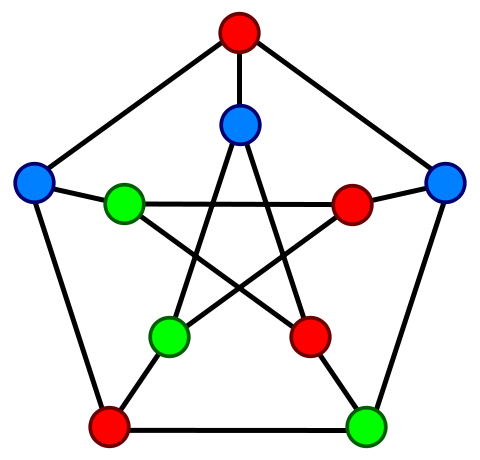
\includegraphics[width=70mm,height=70mm]{graf.png}
\caption{A proper vertex coloring of the Petersen graph with 3 colors, the minimum number possible. \label{overflow}}
\end{figure}

\begin{figure}[ht!]
\centering
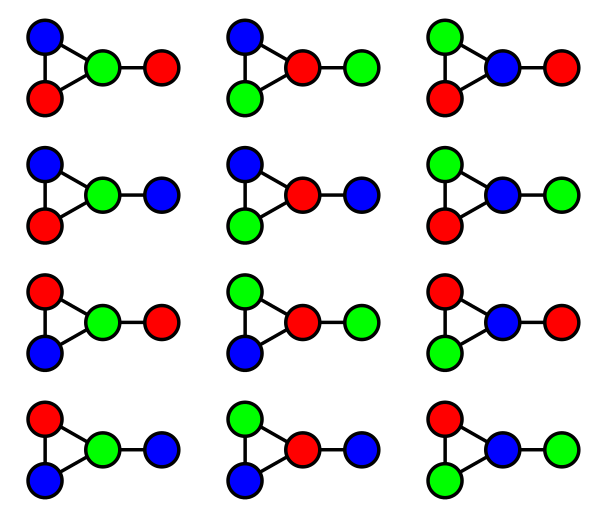
\includegraphics[width=60mm,height=60mm]{graf1.png}
\caption{This graph can be 3-colored in 12 different ways.
 \label{overflow}}
\end{figure}


\section{Descrierea aplicatiei}
Pentru a reprezenta un graf, într-un program, am folosit structuri de date ce reprezinta graful prin matricea de adiacentă , o matrice patratica in care adiacenta dintre 2 noduri este notata cu 1, iar in caz contrar cu 0 . Colorarea grafului si aflarea numarului cromatic se face folosind 2 algoritmi (Greedy si Backtracking). Am creat functii pentru rezolvarea fiecarui algoritm.
Pentru realizarea grafului , am folosit structura:
\begin{itemize}
  \item [i)]{\bf struct a-graph},cu ajutorul careia am definit numarul nodurilor,initializarea grafului si matricea de adiacenta.Structura contine:numarul de noduri(int no-nodes),initializarea(int init) si un pointer catre matricea de adiacenta (int *adj-matrix).
\end{itemize}
In continuare,am definit functii pentru citirea matricei de adiacenta atat de la tastatura cat si din fisier astfel :
\begin{itemize}
  \item [i)]Functia\ {\bf set-adj-matrix-value()}, ce seteaza pe pozitia curenta din matrice valoarea 0 sau 1.
  \item [ii)]Functia\ {\bf init-graph()}, ce initializeaza graful citind matricea de adiacenta de la tastatura si o seteaza cu ajutorul functiei set-adj-matrix-value.
  \item [iii)]Functia\ {\bf init-graph-file()}, ce initializeaza graful citind matricea de adiacenta din fisier obtinuta prin generare random a valorilor ( la care vom aveam nevoie de libraria time.h) si scrierea valorilor in fisier, si o seteaza cu ajutorul functiei set-adj-matrix-value.
  \item [iiii)]Functia\ {\bf get-adj-matrix-value()}, ce returneaza valoarea elementului matricei de adiacenta pe pozitia curenta , daca graful este initializat. In caz contrar , returneaza -1.
   \item [iiiii)]Functia\ {\bf print-adj-matrix()}, functie ce afiseaza matricea de adiacenta cu ajutorul functiei get-adj-matrix-value, daca graful este initializat.In caz contrar, afiseaza "Te rog citeste graful mai intai".
  \item [iiiiii)]Functia\ {\bf adj-check()}, care verifica daca 2 noduri sunt adiacente cu ajutorul functiei get-adj-matrix-value, returnand valoarea 1 daca verificarea este adevarata si 0 daca e falsa.
\end{itemize}
Odata initializat graful si cunoscand matricea de adiacenta ,putem construi algoritmii ajutatori rezolvarii problemei:

\pagebreak


Descrierea functiilor principale ale acestui proiect:
\begin{enumerate}
  \item [1.]Functia\ {\bf void chromatic-number-greedy ()} primeste ca parametru structura {\bf struct} a-graph *graph. Aceasta functie rezolva problema prin algoritmul Greedy , care face la nivel local alegerea optimă pentru fiecare etapă în speranța de a găsi un optim global. Pentru inceput se defineste vectorul de marime alocata dinamic in care vor fi stocate culorile necesare si fisierul in care vor fi stocate datele de iesire. Initializam minimul numarului de culori necesare care este 1 deoarece avem nevoie de cel putin o culoare pt a colora un graf, apoi parcugem nodurile grafului cu ajutorul iteratorului $iterator_1$. Initial toate nodurile vor avea culoarea 1, apoi parcurgem toate nodurile de dinaintea iteratorului $iterator_1$ cu ajutorul iteratorului $iterator_2$ si verificam daca cele doua noduri sunt adiacente si au aceeasi culoare.Daca verificarea este adevarata atunci culoarea nodului $iterator_2$ va creste cu 1 , adica nodului ii vom atribui o alta culoare, iar minimul numarului de culori va fi valoarea culorii $iteratorului_2$ crescuta cu 1. Se repeta pana cand gasim un nod $iterator_2$ ce nu are culoarea unui nod adiacent $iterator_1$.\\
  La final parcurgem din nou nodurile si afisam ce culoare i-a fost atribuita fiecarui nod si de asemenea afisam numarul minim de culori necesare ,adica numarul cromatic.
  \item [2.]Functia\ {\bf void print-chromatic-number(int *colors, struct a-graph *graph)}, functie ajutatoare rezolvarii cu metoda Backtracking.Aceasta afiseaza in fisierul unde sunt stocate datele de iesire ce culoare i-a fost atribuita fiecarui nod si numarul minim de culori necesare ,adica numarul cromatic.
  
  \item [3.]Functia\ {\bf int check-same-color(int node, struct a-graph *graph, int *colors, int color)},verifica daca 2 noduri sunt adiacente si au aceeasi culoare.Este de asemenea o functie ajutatoare ce are ca parametrii un nod $node$ si o culoare $color$ si parcurgand nodurile grafului cu ajutorul iteratorului $iterator_1$ , verifica daca nodul $node$ si nodul $iterator_1$ sunt adiacente si culoarea nodului $iterator_1$ este aceesi cu culoarea $color$.Daca este adevarat returneaza 0. Altfel ,returneaza 1.
  
  \item [4.]Functia\ {\bf int recursive-backtracking-coloring(struct a-graph *graph, int max-no-colors, int *colors, int node)} este o functie recursiva ajutatoare colorarii grafului.Verificam daca nodul $node$ a ajuns la final si nu ne-a mai ramas niciun nod, in acest caz returnam 1 ca conditie de oprire. Parcurgand culorile necesare cu ajutorul iteratorului $color_iterator$ pana la valoarea maxima a numarului de culori necesare data ca parametru $max-no-colors$ ,verificam daca nodul $node$ este adiacent cu alt nod din graf si daca culoarea $color_iterator$ este aceeasi , cu alte cuvinte verificam daca ii putem atribui in siguranta nodului $node$ culoarea $color_iterator$. Autoapelam functia pentru a atribui culori pentru restul nodurilor. Cand au fost atribuite culori tuturor nodurilor functia returneaza 1.
  Daca culoarea $color_iterator$ nu poate duce la nicio solutie atunci o eliminam atribuindu-i valoarea 0.
  Ultima conditie de oprire : returneaza 0 cand niciuna dintre conditiile de mai sus nu s-au rulat;
  
  \item [5.]Functia\ {\bf int chromatic-number-backtracking(struct a-graph *graph, int max-no-colors)} rezolva problema prin aloritmul Backtracking bazat pe functiile anterioare la care vom face apel.
  Verficam daca culorile au fost atribuite cu ajutorul functiei recursive-backtracking-coloring(graph, max-no-colors, colors, 0) pornind de la nodul 0. Daca verificarea este falsa atunci nu exista nicio solutie cu conditia de oprire return 0 , altfel, afisam numarul cromatic cu ajutorul functiei print-chromatic-number(colors, graph) avand conditie de oprire return 1.
  
  \item [6.]Functia\ {\bf int main()},cuprinde declararea variabilelor: variabila *graph de tip struct a-graph *graph si variabila pentru a alege ce metoda sa folosim, {\bf int choose-algorithm};variabilei *graph i se aloca dinamic memorie de marimea struct a-graph , variabila prin intermediul careia putem ajunge la nodurile grafului sau la matricea de adiacenta; Urmeaza citirea datelor,care se realizeaza dupa dorinta user-ului, fie de la tastatura fie random din fisierul {\bf in},afisarea realizandu-se in fisierul {\bf out}.\\
  Dupa citire afisam matricea de adiacenta , apoi se realizeaza alegerea algoritmului de rezolvare tot cu ajutorul variabilei $choose-algorithm$. \\
  In final , eliberam memoria utilizata de variabila *graph si de matricea de adiacenta folosind functia predefinita void free (void*ptr) din libraria stdlib.h.

\end{enumerate}
\pagebreak

\section{Concluzii}
La prima vedere,sau mai bine spus,atunci cand citesti prima data cerinta problemei,nu pare deloc complicat,insa din punctul meu de vedere,cel mai greu a fost sa definesc functiile principale si cele ajutatoare ce rezolva problema prin 2 algoritmi.


\section{Bibliografie}

\begin{itemize}
  \item [i)] $The\ C\ Programming\ language,Second Edition$,Bian W. Kernighan,Dennis M. Ritchie
  \item [ii)] $\href{http://ad.becheru.net/}{Programming\ Techniques\ course}$
  \item [iii)] $\href{https://en.wikipedia.org/wiki/Graph_coloring}{Wikipedia}$
   \item [iiii)] $\href{https://www.geeksforgeeks.org/graph-coloring-applications/}{GeeksforGeeks}$
\end{itemize}

\pagebreak
\section{Experimente si rezultate}

Generarea automata non-trivial input test data a fost facuta initializand functia srand((unsigned) time(t)), atribuind random numarul de noduri de la 1 la 5 \leftarrow $1 + rand() modulo 5 , (pentru facilitatea citirii de catre user) si matricea de adiacenta random luand valoarea 0 sau 1 $\leftarrow $(rand() modulo 2)$.\\
$Compararea celor 2 algoritmi:$\\

\begin{figure}[ht!]
\centering
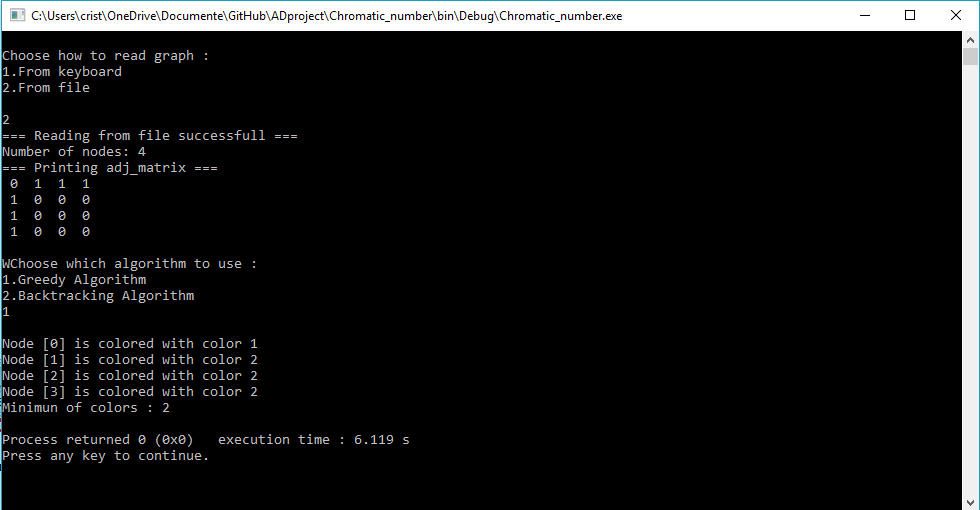
\includegraphics[width=150mm,height=80mm]{testAlgoritm1.png}
\caption{Test random generator Algoritm 1. \label{overflow}}
\end{figure}

\begin{figure}[ht!]
\centering
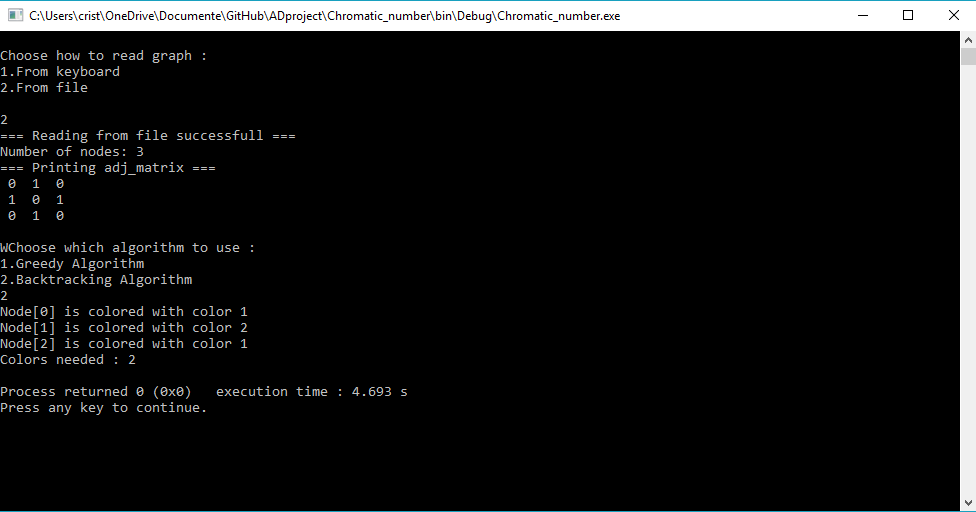
\includegraphics[width=150mm,height=80mm]{testAlgoritm2.png}
\caption{Test random generator Algoritm 2. \label{overflow}}
\end{figure}
\pagebreak
In cazul introducerii unui graf cu 3 noduri in care nodurile 1 si 2 sunt adiacente,rezultatul programului este:
\begin{figure}[ht!]
\centering
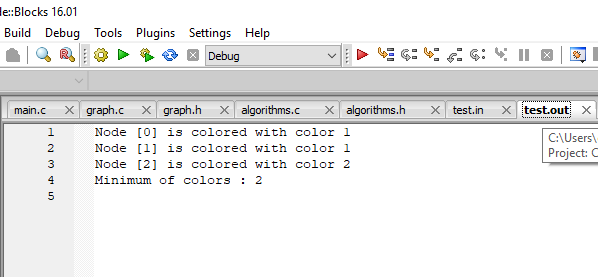
\includegraphics[width=120mm,height=50mm]{test1.png}
\end{figure}



\end{document}